\documentclass[a4paper,titlepage]{article}
\usepackage[utf8]{inputenc}
\usepackage{fullpage}
\usepackage{indentfirst}
\usepackage[per-mode=symbol]{siunitx}
\usepackage{listings}
\usepackage{graphicx}
\usepackage{color}
\usepackage{amsmath}
\usepackage{array}
\usepackage[hidelinks]{hyperref}
\usepackage[format=plain,font=it]{caption}
\usepackage{subcaption}
\usepackage{standalone}
\usepackage[nottoc]{tocbibind}
\usepackage[noabbrev,capitalize,nameinlink]{cleveref}
\usepackage{listings}
\usepackage{titlesec}
\usepackage{minted}
\usepackage{booktabs}
\usepackage{csvsimple}
\usepackage{siunitx}
\usepackage[super]{nth}
\usepackage[titletoc]{appendix}

% Custom commands
\newcommand\numberthis{\addtocounter{equation}{1}\tag{\theequation}}
\newcommand{\code}[1]{\texttt{#1}}
\newcolumntype{P}[1]{>{\centering\arraybackslash}p{#1}}

\setminted{linenos,breaklines,fontsize=auto}

%\titleformat*{\section}{\normalsize\bfseries}
%\titleformat*{\subsection}{\small\bfseries}
\renewcommand{\thesubsection}{\thesection.\alph{subsection}}
\providecommand*{\listingautorefname}{Listing}
\newcommand*{\Appendixautorefname}{Appendix}

%opening
\title{\textbf{ECSE 543 \\ Assignment 1}}
\author{Sean Stappas \\ 260639512}
\date{October \nth{21}, 2017}

\begin{document}
	\sloppy
	\maketitle
	
	\tableofcontents
	
	
	\twocolumn
	
	\section*{Introduction}
	
	The code for this assignment was created in Python 2.7 and can be seen in \autoref{appendix:code}. To perform the required tasks in this assignment, a custom \mintinline{python}{Matrix} class was created, with useful methods such as add, multiply, transpose, etc. This package can be seen in the \mintinline{python}{matrices.py} file shown in \autoref{lst:matrices}. The structure of the rest of the code will be discussed as appropriate for each question. Output logs of the program are provided in \autoref{appendix:logs}.
	
	The only packages used that are not built-in are those for fitting curves and creating the plots for this report. These include \mintinline{python}{matplotlib} for plotting, \mintinline{python}{numpy} for curve fitting and \mintinline{python}{sympy} for printing mathematical symbols on the plots. Curve fitting was used to fit the $R(N)$ function in Question 2 and to fit polynomial complexity functions to the number of iterations or runtime of various parts of the program. For any curve fit, the fitting function is given in the legend of the associated plot.
	
	\section{Choleski Decomposition}
	
	The source code for the Question 1 program can be seen in the \mintinline{python}{q1.py} file, shown in \autoref{lst:q1}.
	
	\subsection{Choleski Program}
	% Write a program to solve the matrix equation Ax=b by Choleski decomposition. A is a real, symmetric, positive-definite matrix of order n.
	
	The code relating specifically to Choleski decomposition can be seen in the \mintinline{python}{choleski.py} file shown in \autoref{lst:choleski}. It is separated into \mintinline{python}{elimination} and \mintinline{python}{back_substitution} methods.
	
	
	\subsection{Constructing Test Matrices}
	% Construct some small matrices (n = 2, 3, 4, or 5) to test the program. Remember that the matrices must be real, symmetric and positive-definite. Explain how you chose the matrices.
	
	The matrices were constructed with the knowledge that, if $A$ is positive-definite, then $A = LL^T$ where L is a lower triangular non-singular matrix. The task of choosing valid $A$ matrices then boils down to finding non-singular lower triangular $L$ matrices. To ensure that $L$ is non-singular, one must simply choose nonzero values for the main diagonal. The Choleski decomposition algorithm then validates that the matrix is positive definite during the elimination phase, throwing an error if it is not.
	
	\subsection{Test Runs}
	% Test the program you wrote in (a) with each small matrix you built in (b) in the following way: invent an x, multiply it by A to get b, then give A and b to your program and check that it returns x correctly.
	
	The matrices were tested by inventing $x$ matrices, and checking that the program solves for that $x$ correctly. The output of the program, comparing expected and obtained values of $x$, can be seen in \autoref{lst:q1_log}.
	
	\subsection{Linear Networks}
	% Write a program that reads from a file a list of network branches (Jk, Rk, Ek) and a reduced incidence matrix, and finds the voltages at the nodes of the network. Use the code from part (a) to solve the matrix problem. Explain how the data is organized and read from the file. Test the program with a few small networks that you can check by hand. Compare the results for your test circuits with the analytical results you obtained by hand. Cleary specify each of the test circuits used with a labeled schematic diagram.
	
	The code relating to solving linear networks can be found in the \mintinline{python}{linear_networks.py} file and is shown in \autoref{lst:linear_networks}. Here, the \mintinline{python}{csv_to_network_branch_matrices} method script reads from a CSV file where row $k$ contains the $J_k$, $R_k$ and $E_k$ values. It then converts the resistances to a diagonal admittance matrix $Y$ and produces the $J$ and $E$ column vectors. The incidence matrix $A$ is also read directly from file, as seen in \autoref{lst:q1}.
	
	First, the program was tested various circuits. These circuits are labeled 1 to 6 and can be seen in \cref{fig:q1_circuit_1,fig:q1_circuit_2,fig:q1_circuit_3,fig:q1_circuit_4,fig:q1_circuit_5,fig:q1_circuit_6}. The corresponding voltages solved by SPICE at each node can be seen in \cref{table:q1_circuit_1,table:q1_circuit_2,table:q1_circuit_3,table:q1_circuit_4,table:q1_circuit_5,table:q1_circuit_6}. Each circuit has corresponding incidence matrix and network branch CSV files, located in the \mintinline{python}{network_data} directory. For each circuit, the program obtains the expected voltages, as seen in the output in \autoref{lst:q1_log}.
	
	% TODO: Add listings of program output here?
	
	\begin{figure}[!htb]
		\centering
		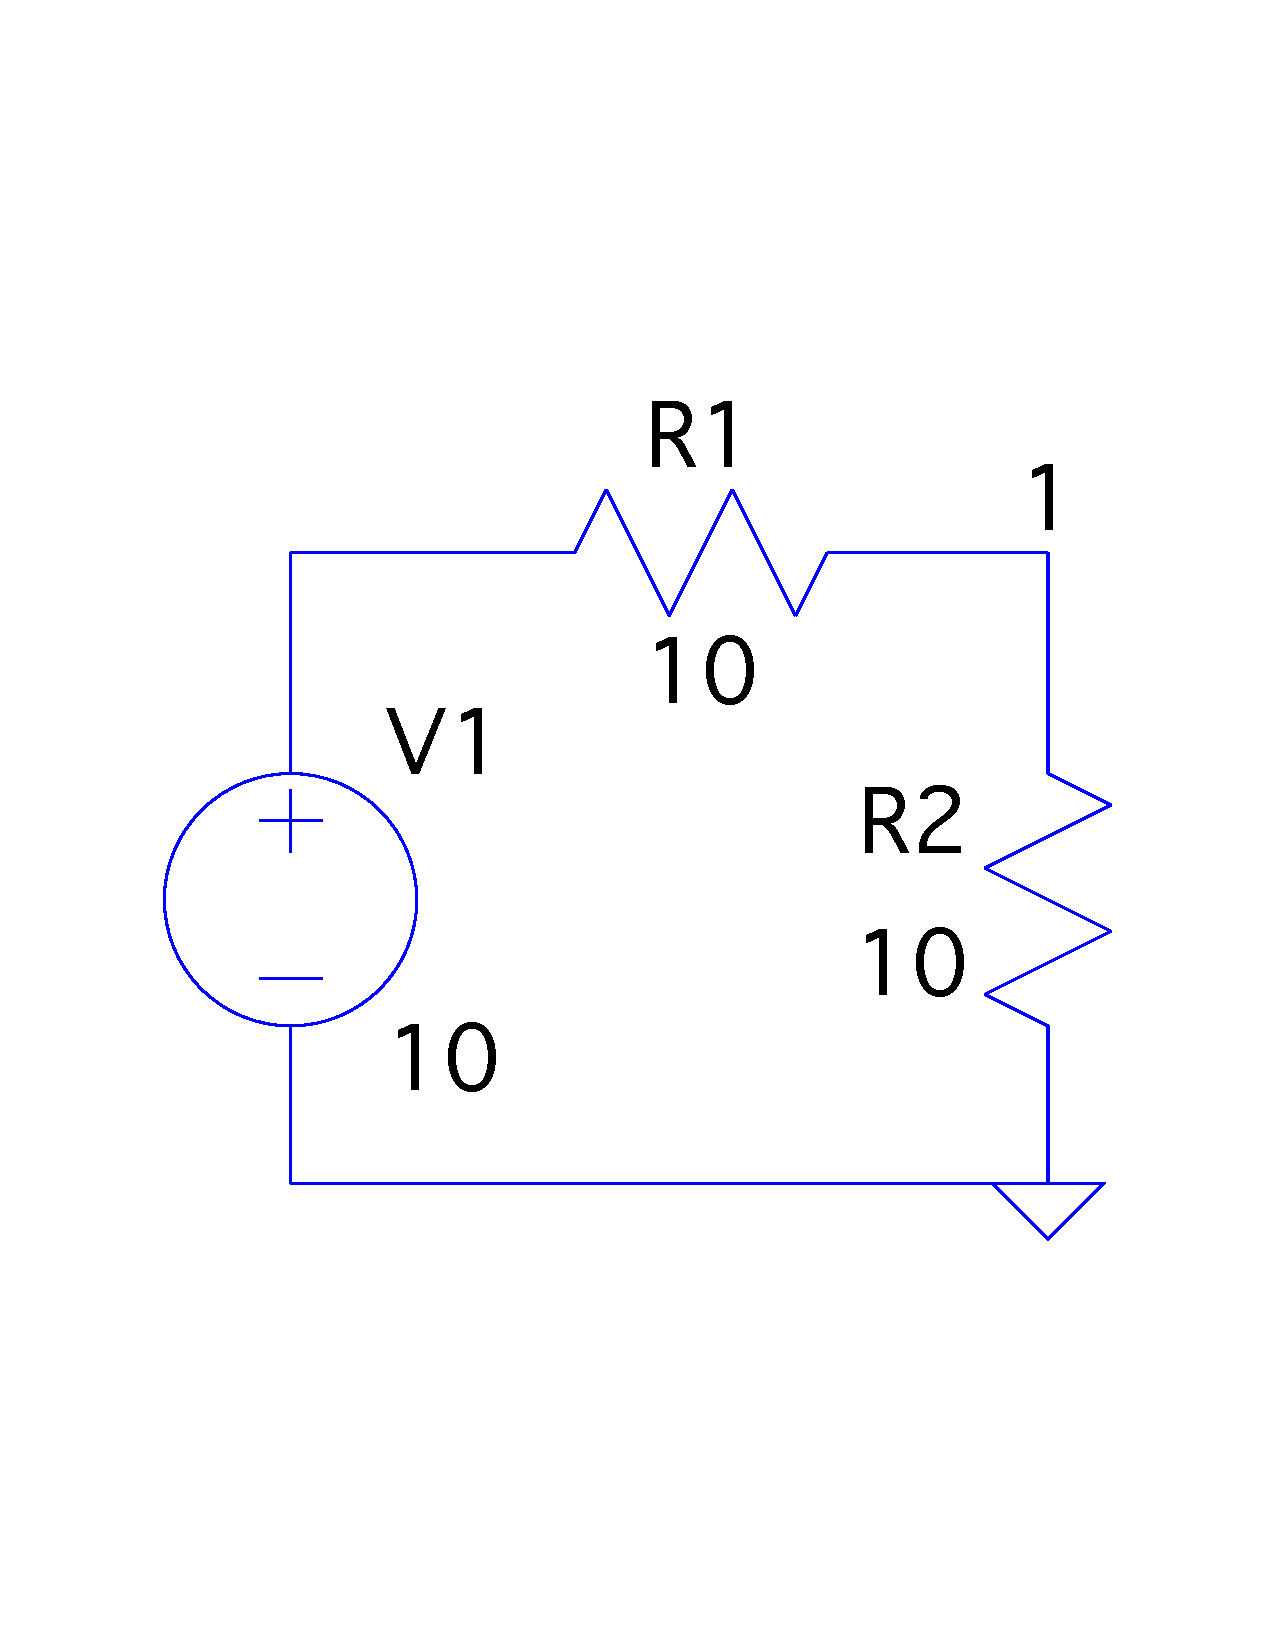
\includegraphics[width=0.5\columnwidth]{plots/q1_circuit_1.pdf}
		\caption
		{Test circuit 1 with labeled nodes.}
		\label{fig:q1_circuit_1}
	\end{figure}

	\begin{table}[!htb]
		\centering
		\caption{Voltage at labeled nodes of circuit 1.}
		\csvautobooktabular{csv/q1_circuit_1.csv}
		\label{table:q1_circuit_1}
	\end{table}

	\begin{figure}[!htb]
		\centering
		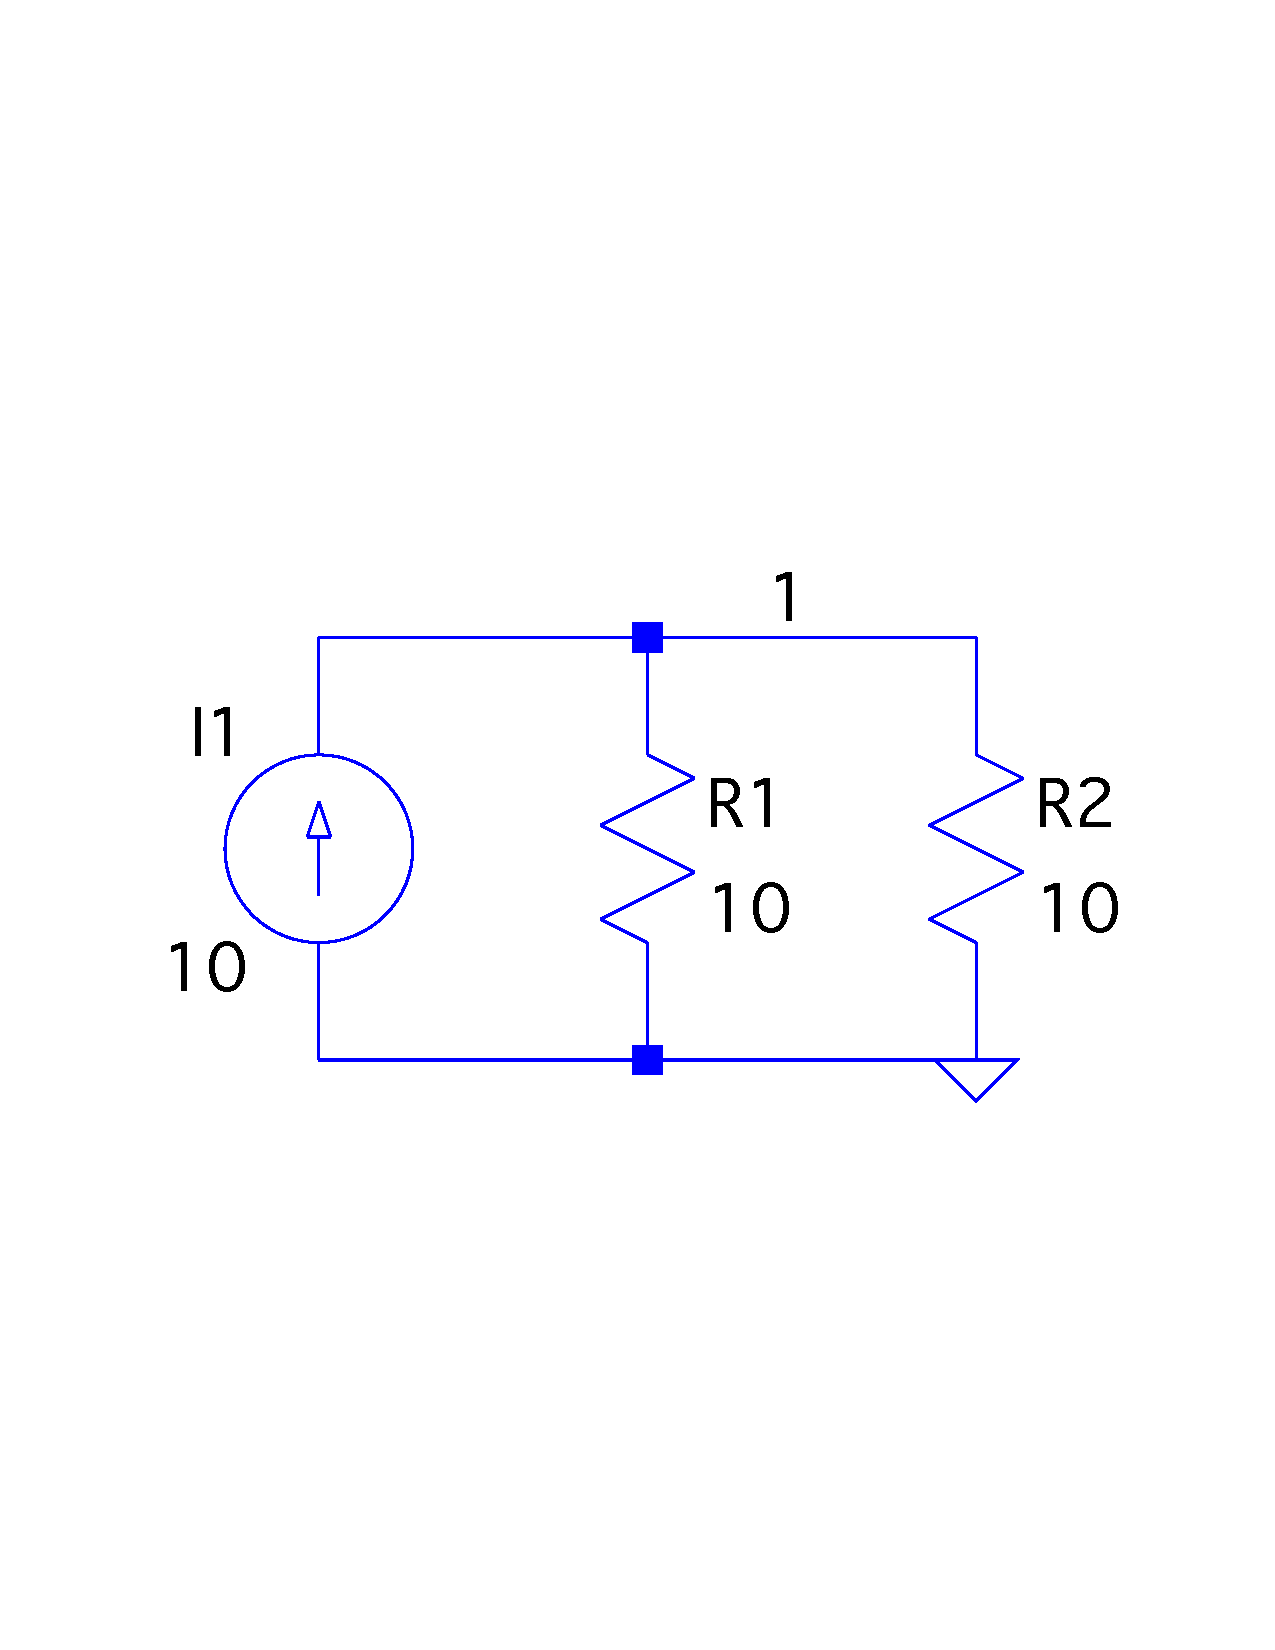
\includegraphics[width=0.5\columnwidth]{plots/q1_circuit_2.pdf}
		\caption
		{Test circuit 2 with labeled nodes.}
		\label{fig:q1_circuit_2}
	\end{figure}
	
	\begin{table}[!htb]
		\centering
		\caption{Voltage at labeled nodes of circuit 2.}
		\csvautobooktabular{csv/q1_circuit_2.csv}
		\label{table:q1_circuit_2}
	\end{table}
	
	\begin{figure}[!htb]
		\centering
		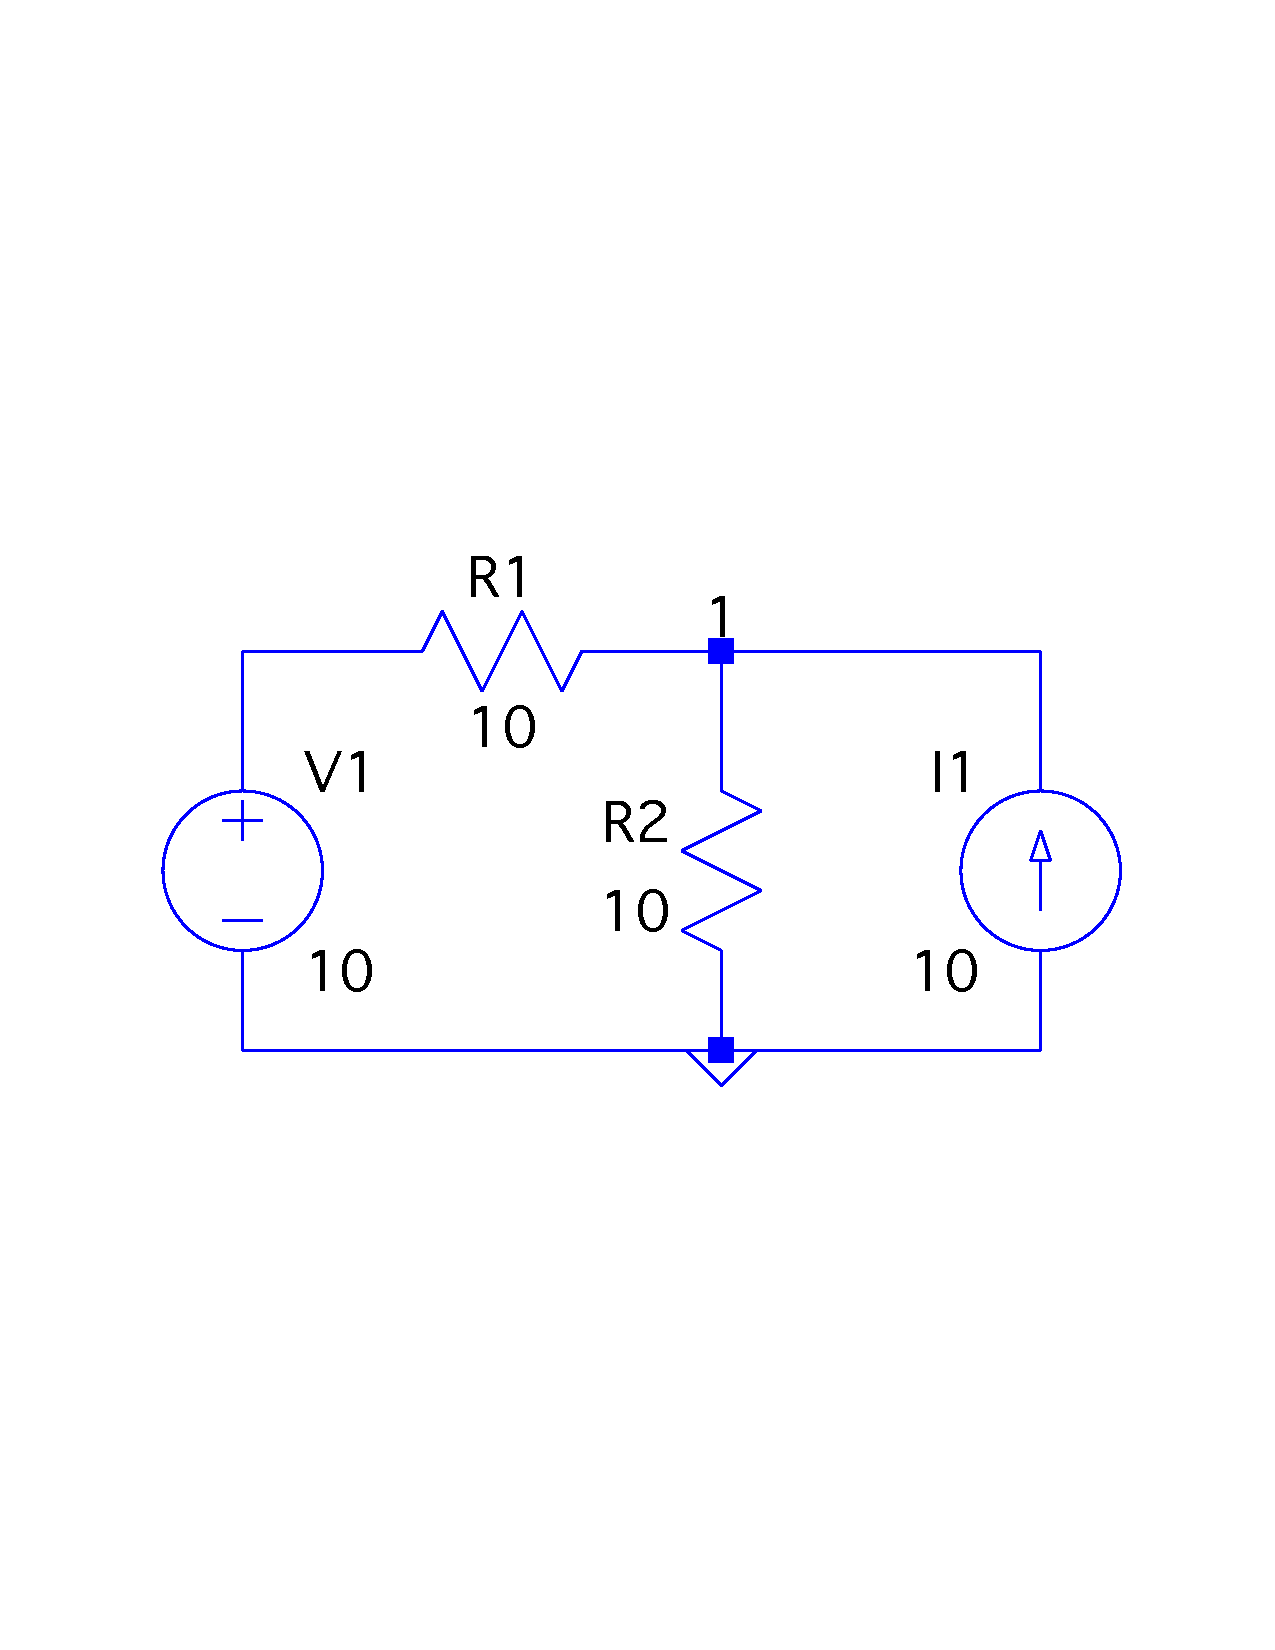
\includegraphics[width=0.5\columnwidth]{plots/q1_circuit_3.pdf}
		\caption
		{Test circuit 3 with labeled nodes.}
		\label{fig:q1_circuit_3}
	\end{figure}
	
	\begin{table}[!htb]
		\centering
		\caption{Voltage at labeled nodes of circuit 3.}
		\csvautobooktabular{csv/q1_circuit_3.csv}
		\label{table:q1_circuit_3}
	\end{table}
	
	\begin{figure}[!htb]
		\centering
		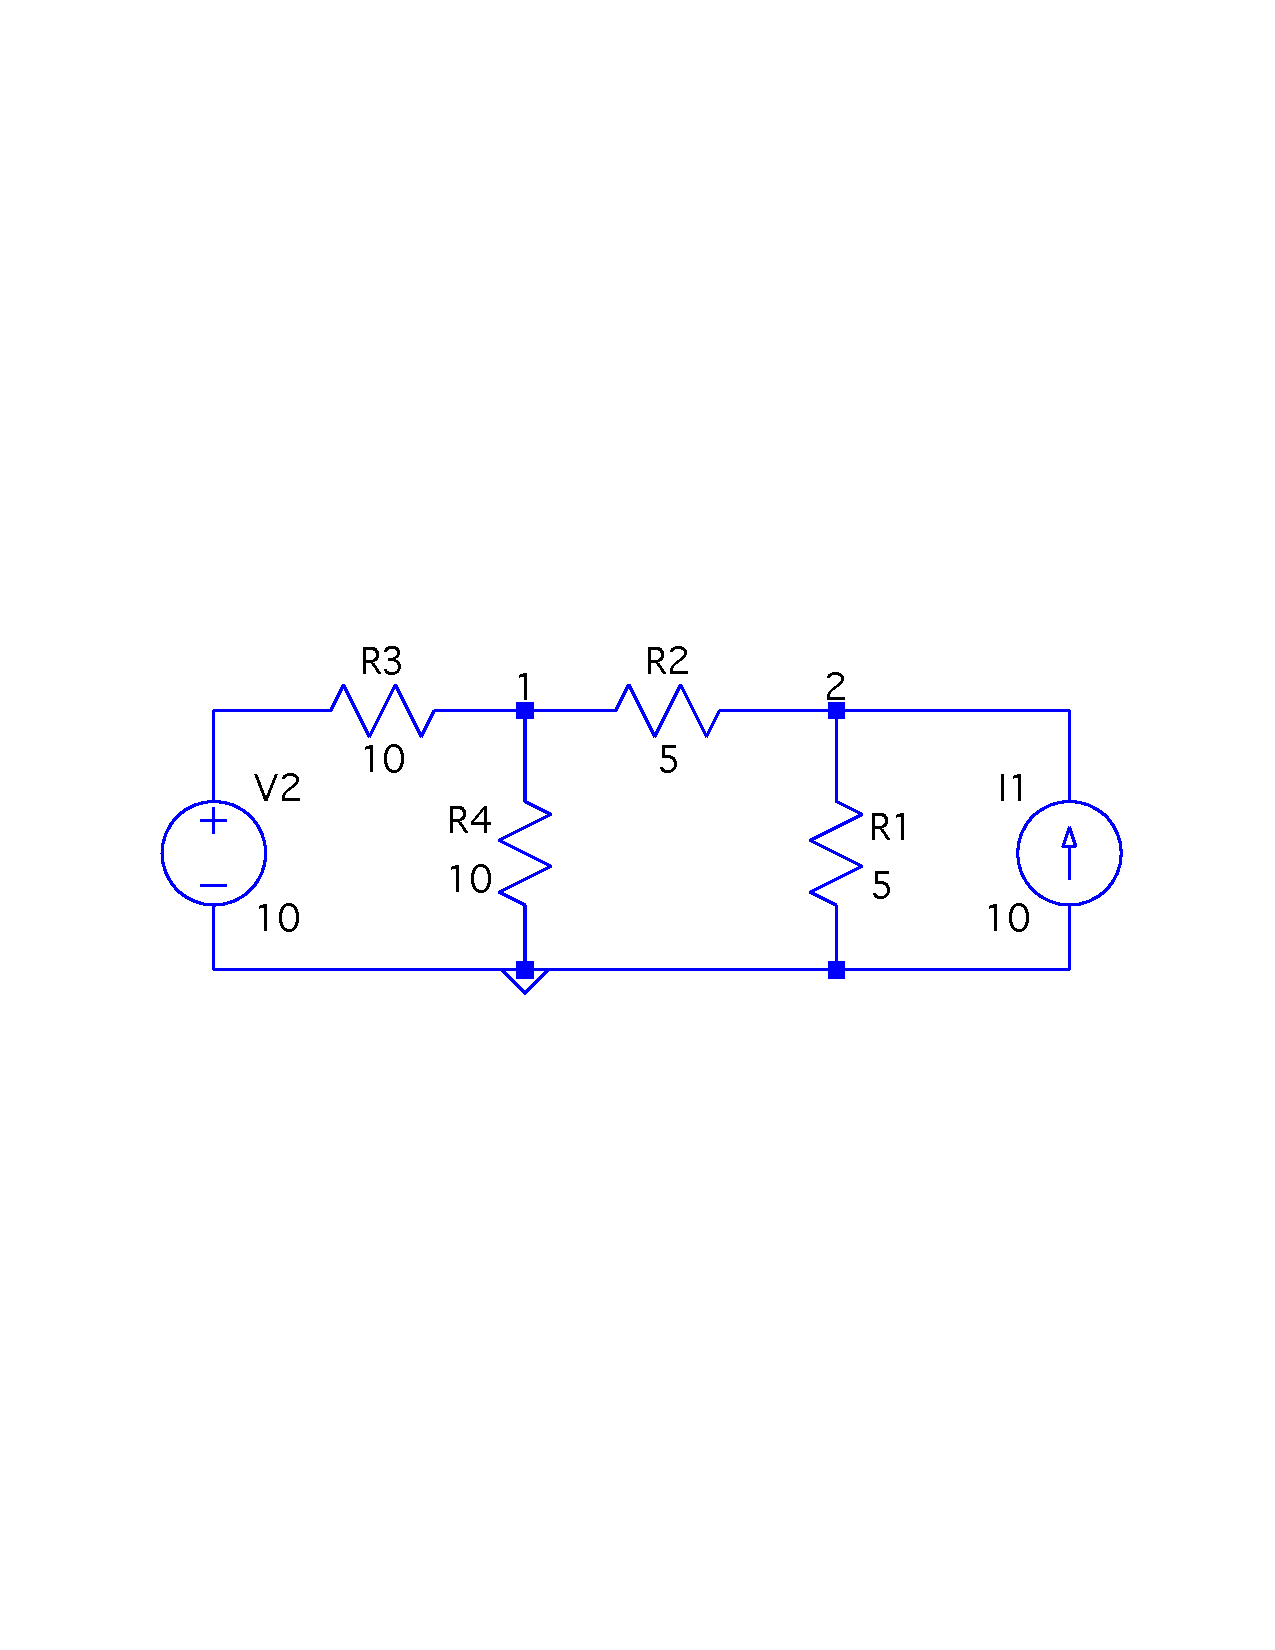
\includegraphics[width=0.75\columnwidth]{plots/q1_circuit_4.pdf}
		\caption
		{Test circuit 4 with labeled nodes.}
		\label{fig:q1_circuit_4}
	\end{figure}
	
	\begin{table}[!htb]
		\centering
		\caption{Voltage at labeled nodes of circuit 4.}
		\csvautobooktabular{csv/q1_circuit_4.csv}
		\label{table:q1_circuit_4}
	\end{table}
	
	\begin{figure}[!htb]
		\centering
		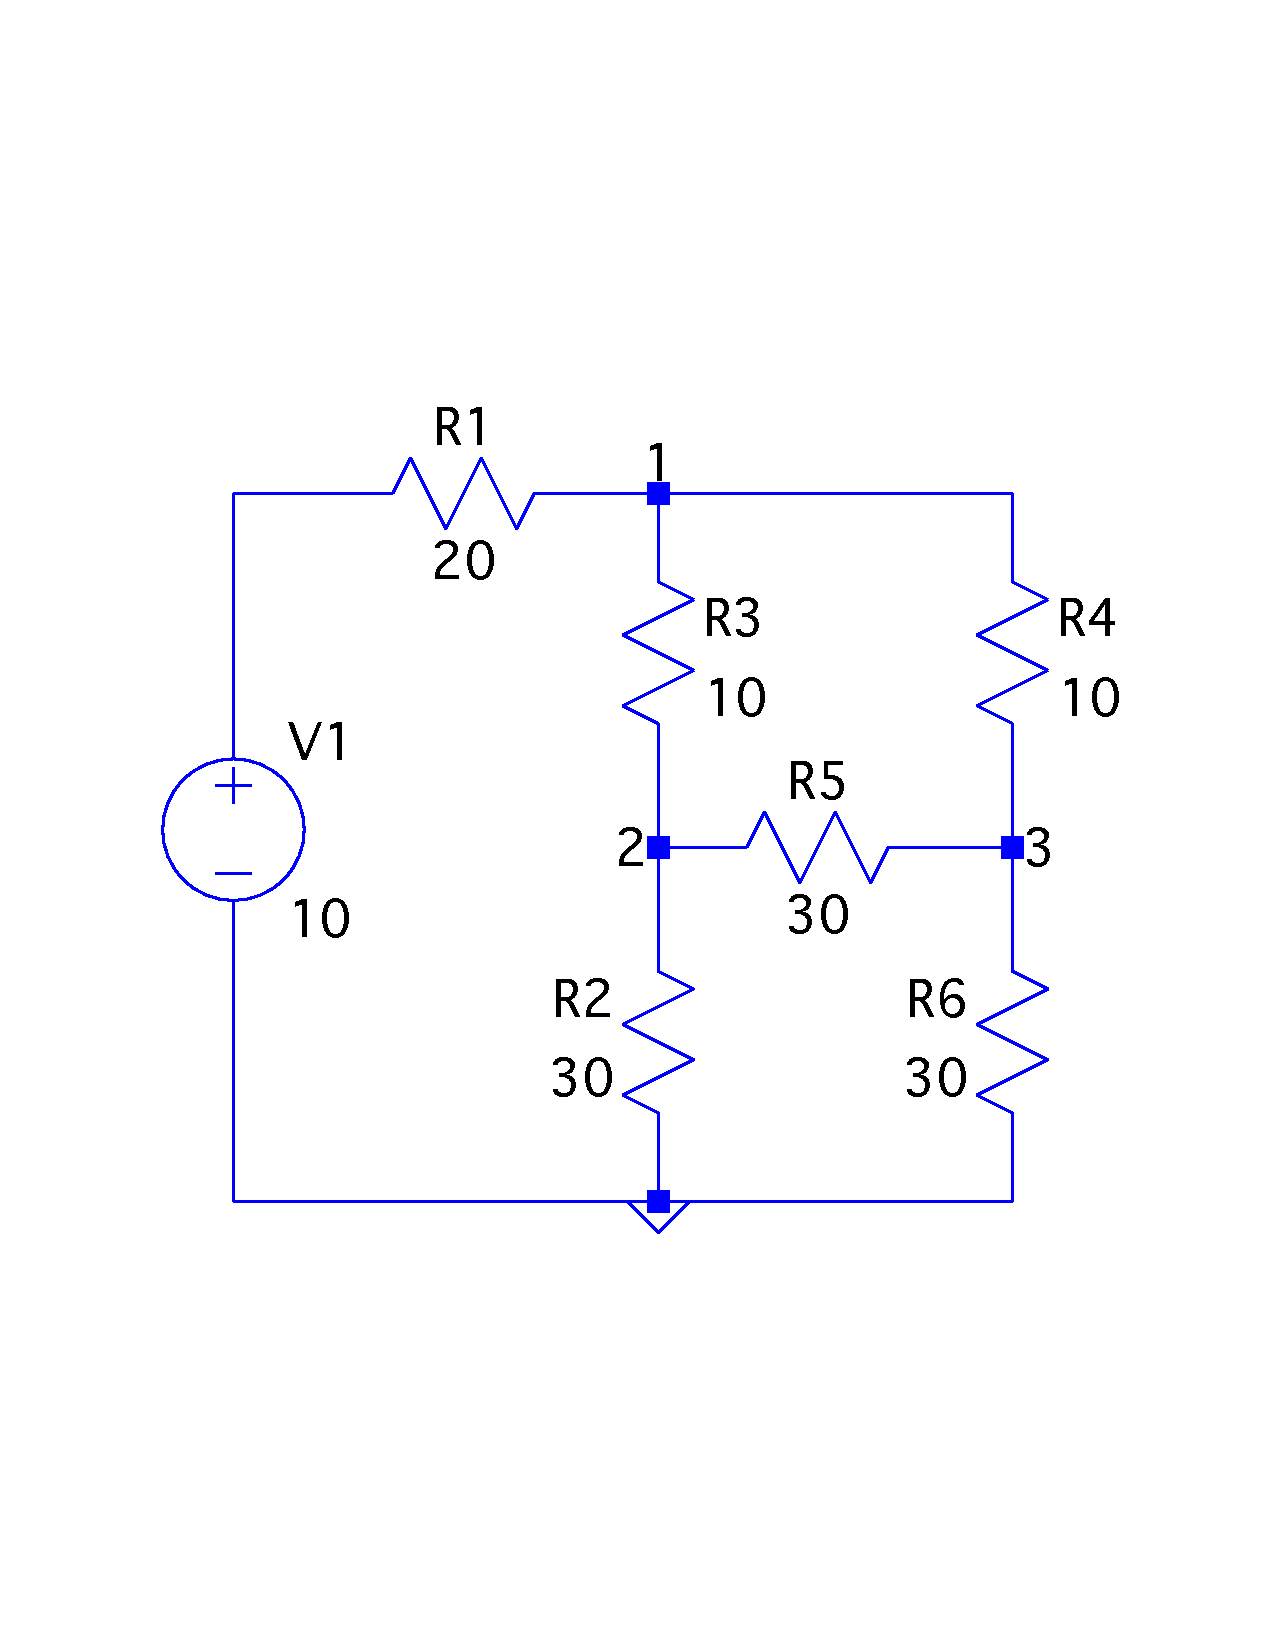
\includegraphics[width=0.75\columnwidth]{plots/q1_circuit_5.pdf}
		\caption
		{Test circuit 5 with labeled nodes.}
		\label{fig:q1_circuit_5}
	\end{figure}
	
	\begin{table}[!htb]
		\centering
		\caption{Voltage at labeled nodes of circuit 5.}
		\csvautobooktabular{csv/q1_circuit_5.csv}
		\label{table:q1_circuit_5}
	\end{table}
	
	\begin{figure}[!htb]
		\centering
		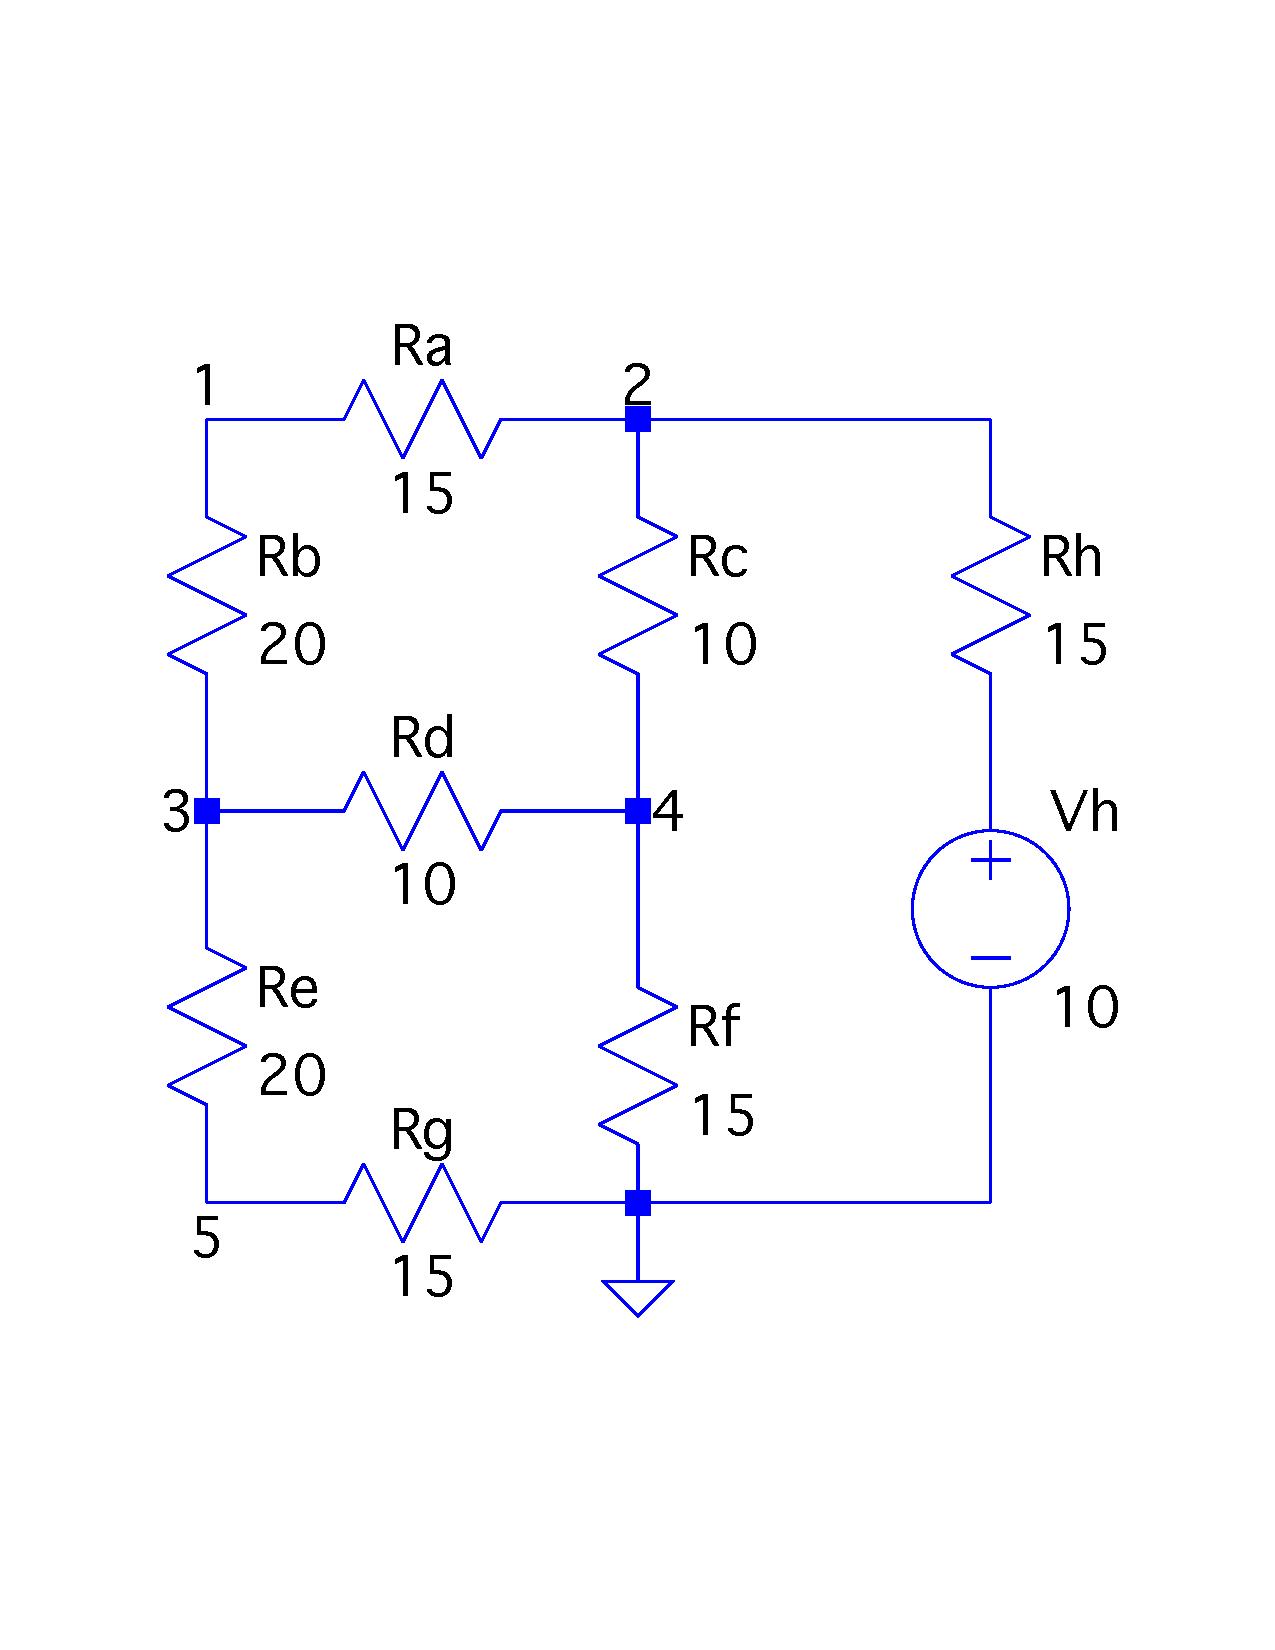
\includegraphics[width=0.75\columnwidth]{plots/q1_circuit_6.pdf}
		\caption
		{Test circuit 6 with labeled nodes.}
		\label{fig:q1_circuit_6}
	\end{figure}

	\begin{table}[!htb]
		\centering
		\caption{Voltage at labeled nodes of circuit 6.}
		\csvautobooktabular{csv/q1_circuit_6.csv}
		\label{table:q1_circuit_6}
	\end{table}
	
	\section{Finite Difference Resistive Mesh}
	
	The source code for the Question 2 program can be seen in the \mintinline{python}{q2.py} file shown in \autoref{lst:q2}.
	
	\subsection{Equivalent Resistance}
	% Using the program you developed in question 1, find the resistance, R, between the node at the bottom left corner of the mesh and the node at the top right corner of the mesh, for N = 2, 3, …, 10. (You will probably want to write a small program that generates the input file needed by the network analysis program. Constructing by hand the incidence matrix for a 200-node network is rather tedious).
	
	The code for creating all the network matrices and for finding the equivalent resistance of an $N$ by $2N$ mesh can be seen in the \mintinline{python}{linear_networks.py} file shown in \autoref{lst:linear_networks}. The \mintinline{python}{create_network_matrices_mesh} method creates the incidence matrix $A$, the admittance matrix $Y$, the current source matrix $J$ and the voltage source matrix $E$. The matrix $A$ is created by reading the associated numbered \mintinline{python}{incidence_matrix} CSV files inside the \mintinline{python}{network_data} directory. Similarly, the $Y$, $J$ and $E$ matrices are created by reading the \mintinline{python}{network_branches} CSV files in the same directory. Each of these files contains a list of network branches $(J_k, R_k, E_k)$. The resistances found by the program for values of $N$ from 2 to 10 can be seen in \autoref{table:q2a}.
	
	\begin{table}[!htb]
		\centering
		\caption{Mesh equivalent resistance R versus mesh size N.}
		\csvautobooktabular{csv/q2a.csv}
		\label{table:q2a}
	\end{table}

	The resistance values returned by the program for small meshes were validated using simple SPICE circuits. The voltage found at the $V_{test}$ node for the 2x4 mesh shown in \autoref{fig:q2a_mesh_2} is \SI{1.875}{\volt} and the equivalent resistance is therefore \SI{1875}{\ohm}. Similarly, for the 3x6 mesh
	 (\autoref{fig:q2a_mesh_3}), $V_{test} = \SI{2.37955}{\volt}$ and the equivalent resistance is \SI{2379.55}{\ohm}. These match the results found by the program, as seen in \autoref{table:q2a}. Bigger mesh circuits were not tested, but these results give at least some confidence that the program is working correctly.
	
	\begin{figure}[!htb]
		\centering
		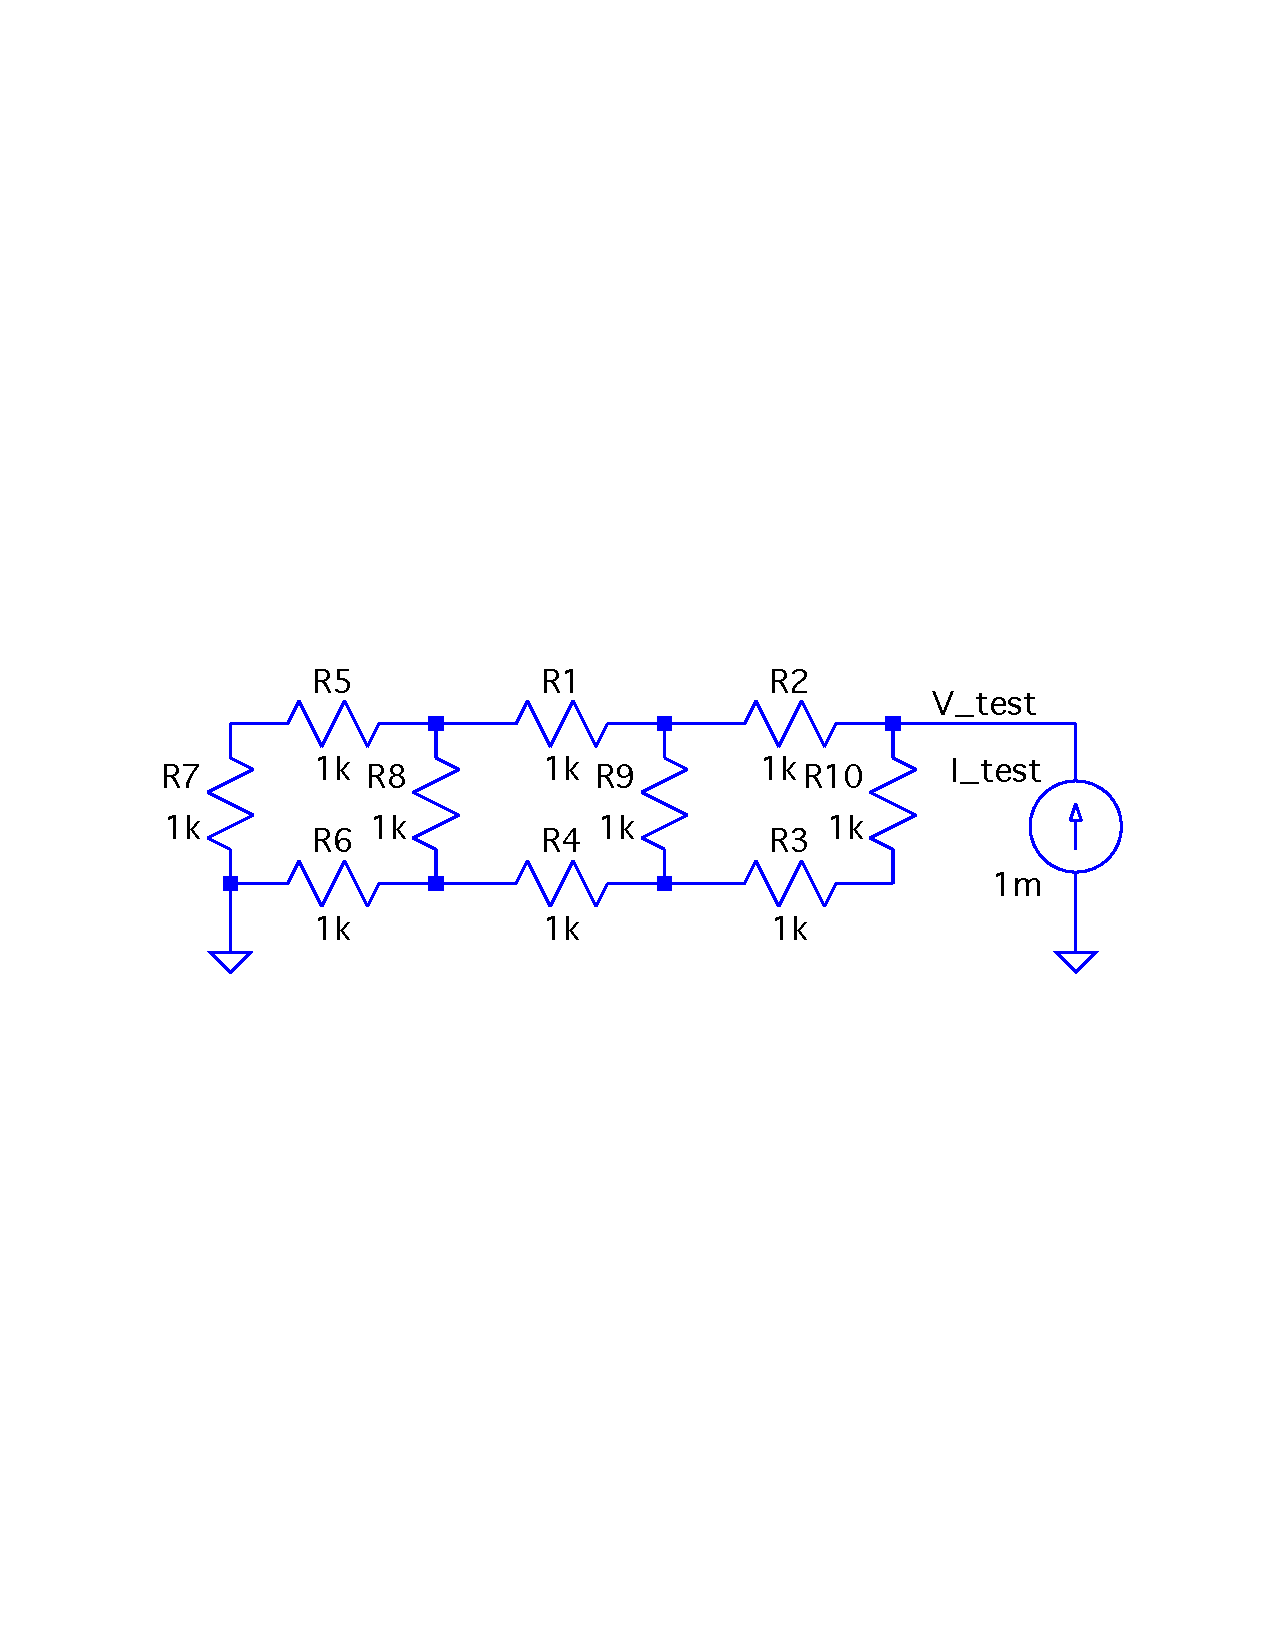
\includegraphics[width=\columnwidth]{plots/q2a_mesh_2.pdf}
		\caption
		{SPICE circuit used to test the 2x4 mesh.}
		\label{fig:q2a_mesh_2}
	\end{figure}

	\begin{figure}[!htb]
		\centering
		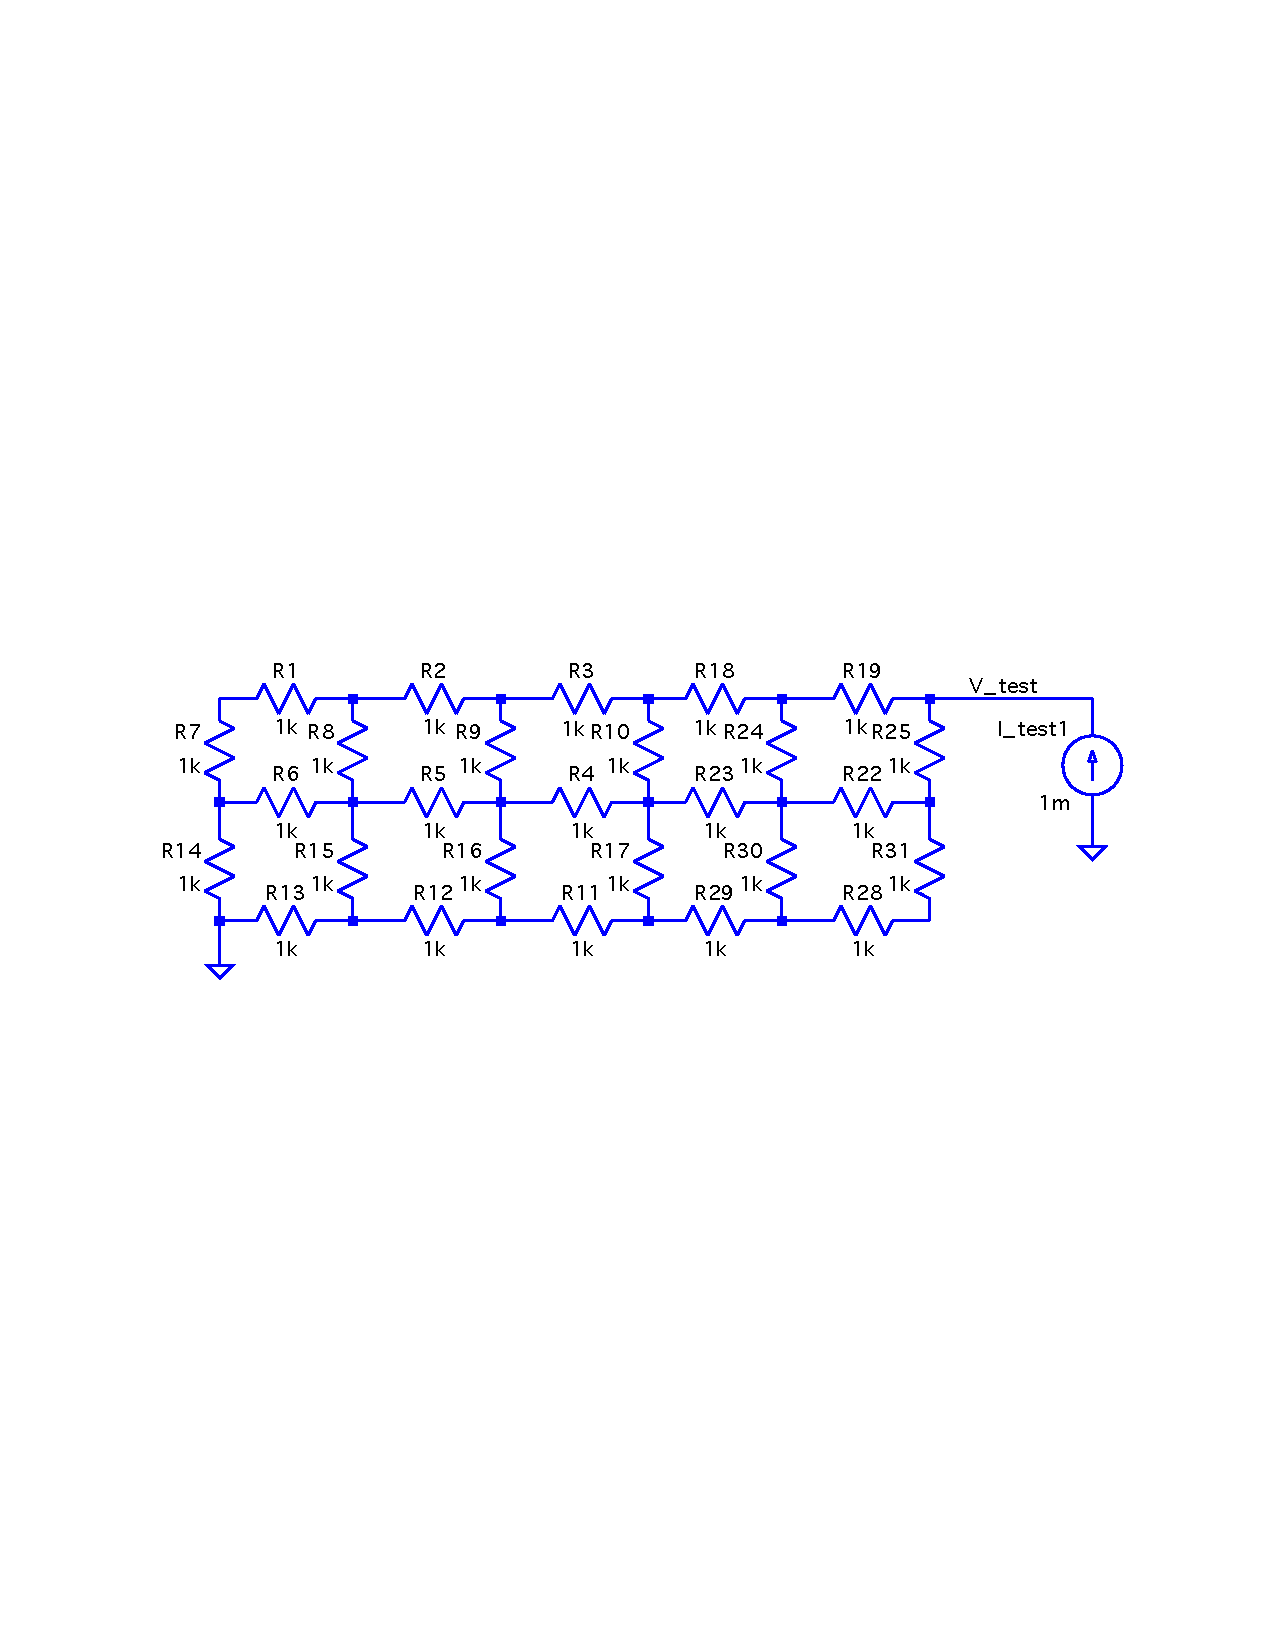
\includegraphics[width=\columnwidth]{plots/q2a_mesh_3.pdf}
		\caption
		{SPICE circuit used to test the 3x6 mesh.}
		\label{fig:q2a_mesh_3}
	\end{figure}
	
	\subsection{Time Complexity}
	% In theory, how does the computer time taken to solve this problem increase with N, for large N? Are the timings you observe for your practical implementation consistent with this? Explain your observations.
	
	The runtime data for the mesh resistance solver is tabulated in \autoref{table:q2b} and plotted in \autoref{fig:q2b}. Theoretically, the time complexity of the program should be $O(N^6)$. However, as can be seen in \autoref{fig:q2b}, $O(N^5)$ more closely matches the obtained data. The simple Choleski program is therefore more efficient than expected. The reasons why are uncertain, but it may be because of successful branch prediction on the repeated zeros of the matrix when performing elimination.
	
	\begin{table}[!htb]
		\centering
		\caption{Runtime of mesh resistance solver program versus mesh size $N$.}
		\csvautobooktabular{csv/q2b.csv}
		\label{table:q2b}
	\end{table}

	\begin{figure}[!htb]
		\centering
		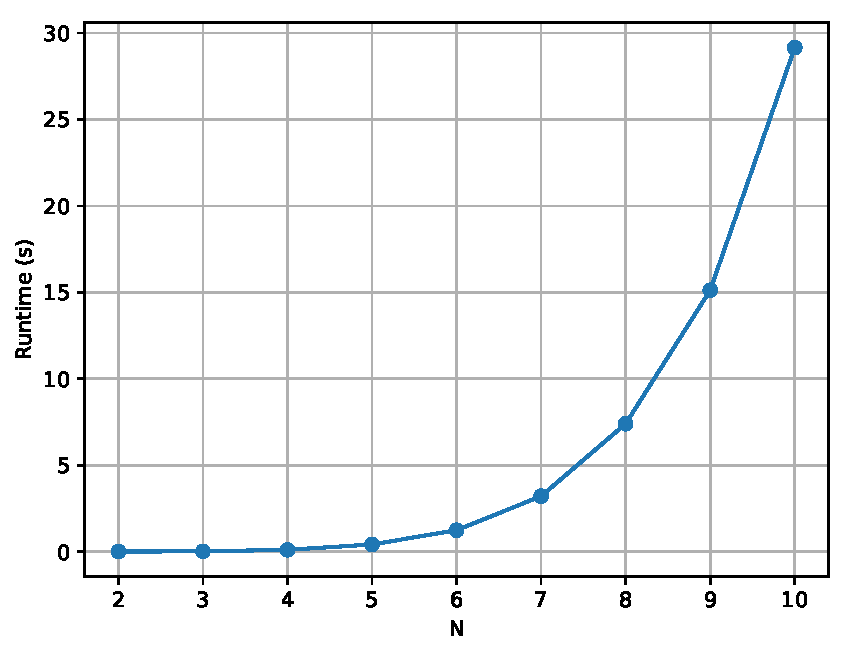
\includegraphics[width=\columnwidth]{plots/q2b.pdf}
		\caption
		{Runtime of mesh resistance solver program versus mesh size $N$.}
		\label{fig:q2b}
	\end{figure}
	
	\subsection{Sparsity Modification}
	% Modify your program to exploit the sparse nature of the matrices to save computation time. What is the half-bandwidth b of your matrices? In theory, how does the computer time taken to solve this problem increase now with N, for large N? Are the timings you for your practical sparse implementation consistent with this? Explain your observations.
	
	The runtime data for the banded mesh resistance solver is tabulated in \autoref{table:q2c} and plotted in \autoref{fig:q2c}. By inspection of the constructed network matrices, a half-bandwidth of $2N + 1$ was chosen. Theoretically, the banded version should have a time complexity of $O(N^4)$, which matches the experimental results.
	
	\begin{table}[!htb]
		\centering
		\caption{Runtime of banded mesh resistance solver program versus mesh size $N$.}
		\csvautobooktabular{csv/q2c.csv}
		\label{table:q2c}
	\end{table}

	\begin{figure}[!htb]
		\centering
		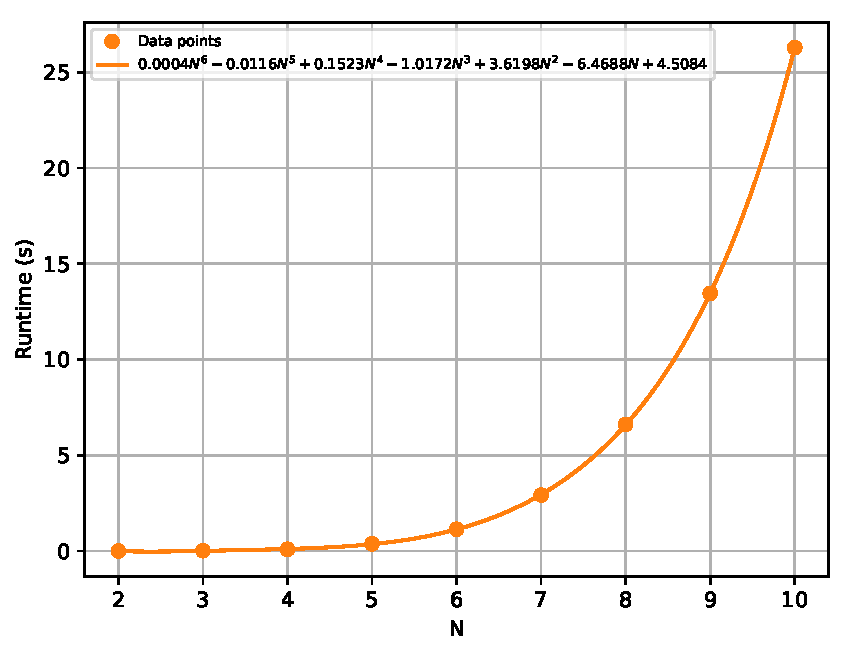
\includegraphics[width=\columnwidth]{plots/q2c.pdf}
		\caption
		{Runtime of banded mesh resistance solver program versus mesh size $N$.}
		\label{fig:q2c}
	\end{figure}

	The runtime of the banded and non-banded versions of the program are plotted in \autoref{fig:q2bc}, showing the marginal benefits of banded elimination. Indeed, the performance increase is not as big as expected, since the non-banded elimination already performed relatively well, possibly because of good branch prediction.

	\begin{figure}[!htb]
		\centering
		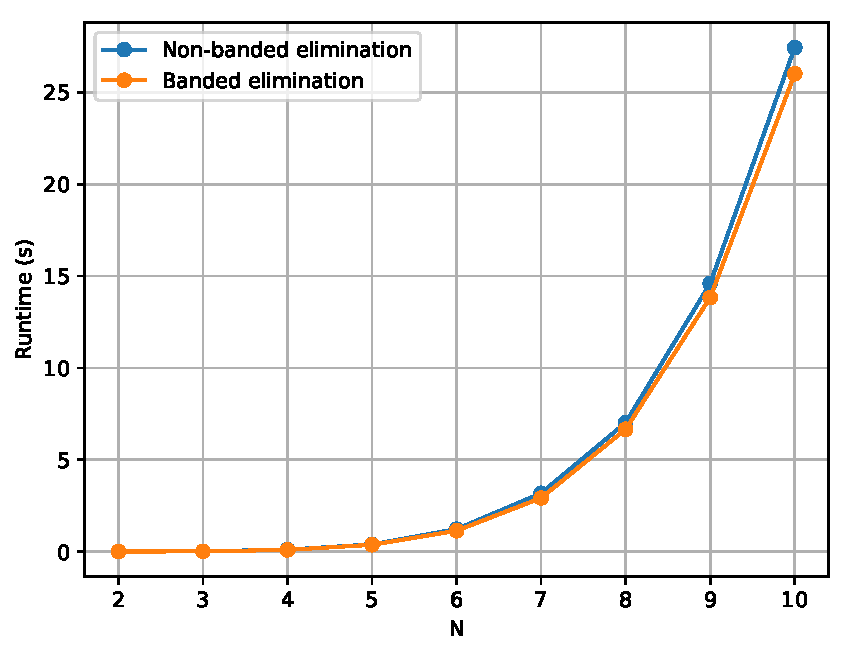
\includegraphics[width=\columnwidth]{plots/q2bc.pdf}
		\caption
		{Comparison of runtime of banded and non-banded resistance solver programs versus mesh size $N$.}
		\label{fig:q2bc}
	\end{figure}
	
	\subsection{Resistance vs. Mesh Size}
	% Plot a graph of R versus N. Find a function R(N) that fits the curve reasonably well and is asymptotically correct as N tends to infinity, as far as you can tell.
	
	The equivalent mesh resistance $R$ is plotted versus the mesh size $N$ in \autoref{fig:q2d}. The function $R(N)$ appears logarithmic, and a log function does indeed fit the data well. As shown in \autoref{fig:q2d}, $R(N) = 1260.81\log{N} + 996.28$ is a good fit, where $R$ is in $\Omega$.
	
	\begin{figure}[!htb]
		\centering
		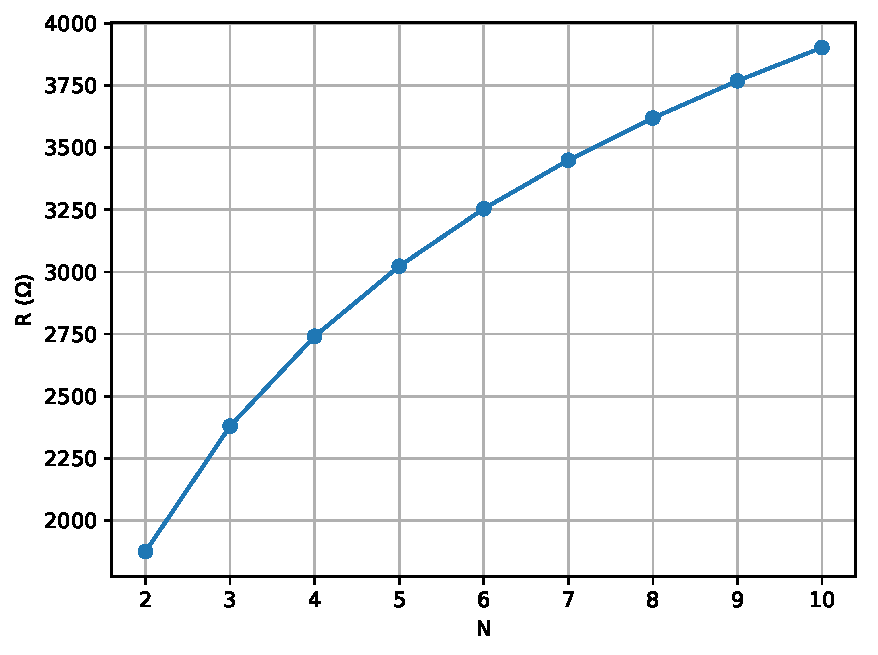
\includegraphics[width=\columnwidth]{plots/q2d.pdf}
		\caption
		{Resistance of mesh versus mesh size $N$.}
		\label{fig:q2d}
	\end{figure}
	
	\section{Coaxial Cable}
	
	The source code for the Question 3 program can be seen in the \mintinline{python}{q3.py} file shown in \autoref{lst:q3}.
	
	\subsection{SOR Program}
	% Write a computer program to find the potential at the nodes of a regular mesh in the air between the conductors by the method of finite differences. Use a five-point difference formula. Exploit at least one of the planes of mirror symmetry that this problem has. Use an	equal node-spacing, h, in the x and y directions. Solve the matrix equation by successive	over-relaxation (SOR), with SOR parameter w. Terminate the iteration when the magnitude	of the residual at each free node is less than 10^-5.
	
	The source code for the finite difference methods can be seen in the \mintinline{python}{finite_diff.py} file shown in \autoref{lst:finite_diff}. Horizontal and vertical symmetries were exploited by only solving for a quarter of the coaxial cable, and reproducing the results where necessary. The initial potential values are guessed based on a radial function from the conductors.
	
	\subsection{Varying $\omega$}
	% With h = 0.02, explore the effect of varying w. For 10 values of w between 1.0 and 2.0,	tabulate the number of iterations taken to achieve convergence, and the corresponding value	of potential at the point (x ,y) = (0.06, 0.04). Plot a graph of number of iterations versus w.
	
	The number of iterations to achieve convergence for 10 values of $\omega$ between 1 and 2 are tabulated in \autoref{table:q3b_iterations} and plotted in \autoref{fig:q3b}. Based on these results, the value of $\omega$ yielding the minimum number of iterations is 1.3.
	
	\begin{table}[!htb]
		\centering
		\caption{Number of iterations of SOR versus $\omega$.}
		\csvautobooktabular{csv/q3b_iterations.csv}
		\label{table:q3b_iterations}
	\end{table}
	
	\begin{figure}[!htb]
		\centering
		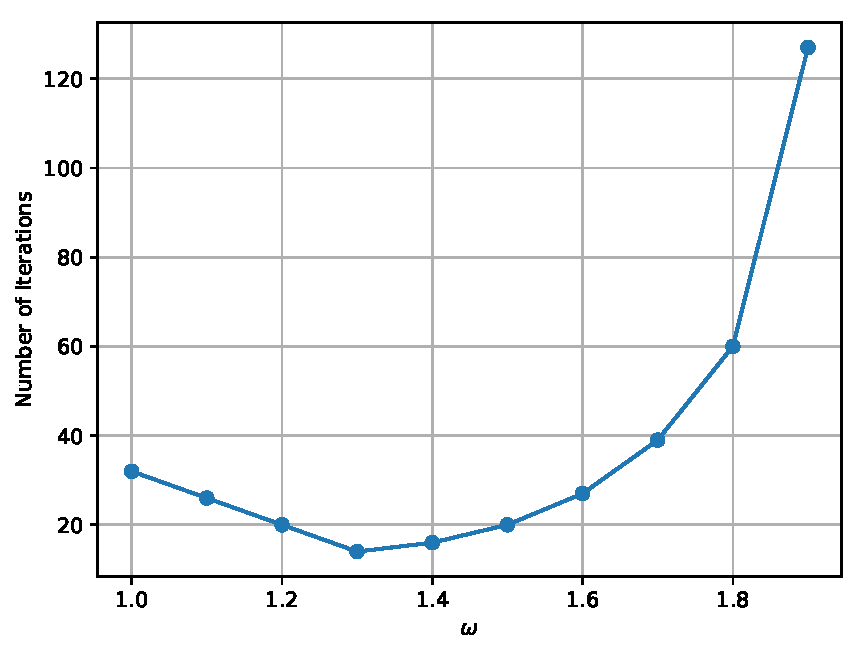
\includegraphics[width=\columnwidth]{plots/q3b.pdf}
		\caption
		{Number of iterations of SOR versus $\omega$.}
		\label{fig:q3b}
	\end{figure}

	The potential values found at (0.06, 0.04) versus $\omega$ are tabulated in \autoref{table:q3b_potential}. It can be seen that all the potential values are identical to 3 decimal places, which shows that the program is converging correctly.

	\begin{table}[!htb]
		\centering
		\caption{Potential at (0.06, 0.04) versus $\omega$ when using SOR.}
		\csvautobooktabular{csv/q3b_potential.csv}
		\label{table:q3b_potential}
	\end{table}
	
	\subsection{Varying $h$}
	% With an appropriate value of w, chosen from the above experiment, explore the effect of	decreasing h on the potential. Use values of h = 0.02, 0.01, 0.005, etc, and both tabulate and	plot the corresponding values of potential at (x, y) = (0.06, 0.04) versus 1/h. What do you think is the potential at (0.06, 0.04), to three significant figures? Also, tabulate and plot the number of iterations versus 1/h. Comment on the properties of both plots.
	
	With $\omega = 1.3$, the number of iterations of SOR versus $1/h$ is tabulated in \autoref{table:q3c_iterations} and plotted in \autoref{fig:q3c_iterations}. It can be seen that the smaller the node spacing is, the more iterations the program will take to run. Theoretically, the time complexity of the program should be $O(N^3)$, where the finite difference mesh is NxN. However, the experimental data shows a complexity closer to $O(1/h^2) = O(N^2)$. The discrepancy can perhaps be because of the relatively small amount of data points.
	
	\begin{table}[!htb]
		\centering
		\caption{Number of iterations of SOR versus $1/h$. Note that $\omega=1.3$.}
		\csvautobooktabular{csv/q3c_iterations.csv}
		\label{table:q3c_iterations}
	\end{table}
	
	\begin{figure}[!htb]
		\centering
		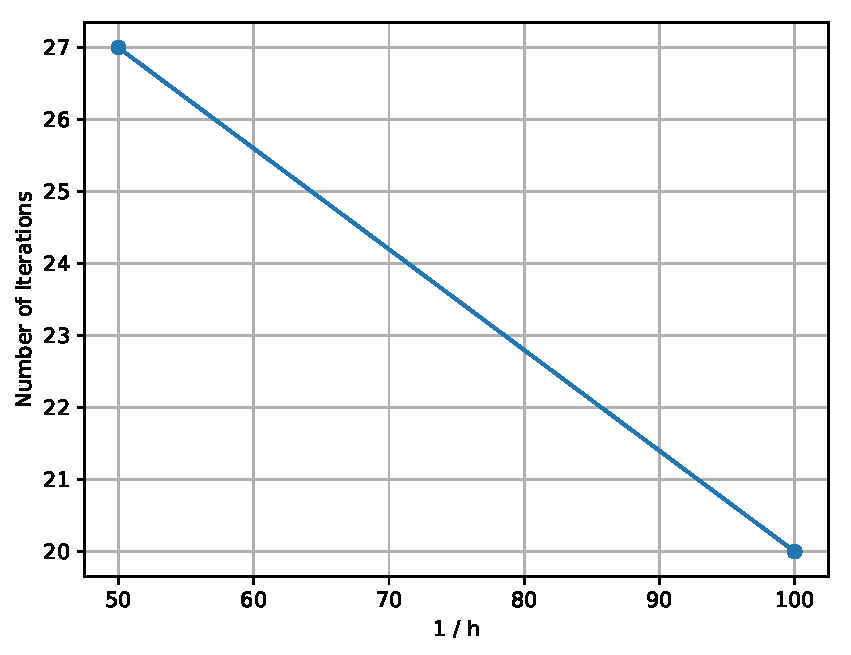
\includegraphics[width=\columnwidth]{plots/q3c_iterations.pdf}
		\caption
		{Number of iterations of SOR versus $1/h$. Note that $\omega=1.3$.}
		\label{fig:q3c_iterations}
	\end{figure}

	The potential values found at (0.06, 0.04) versus $1/h$ are tabulated in \autoref{table:q3c_potential} and plotted in \autoref{fig:q3c_potential}. By examining these values, the potential at (0.06, 0.04) to three significant figures is approximately \SI{5.25}{\volt}. It can be seen that the smaller the node spacing is, the more accurate the calculated potential is. However, by inspecting \autoref{fig:q3c_potential} it is apparent that the potential converges relatively quickly to around \SI{5.25}{\volt}. There are therefore diminishing returns to decreasing the node spacing too much, since this will also greatly increase the runtime of the program.

	\begin{table}[!htb]
		\centering
		\caption{Potential at (0.06, 0.04) versus $1/h$ when using SOR.}
		\csvautobooktabular{csv/q3c_potential.csv}
		\label{table:q3c_potential}
	\end{table}

	\begin{figure}[!htb]
		\centering
		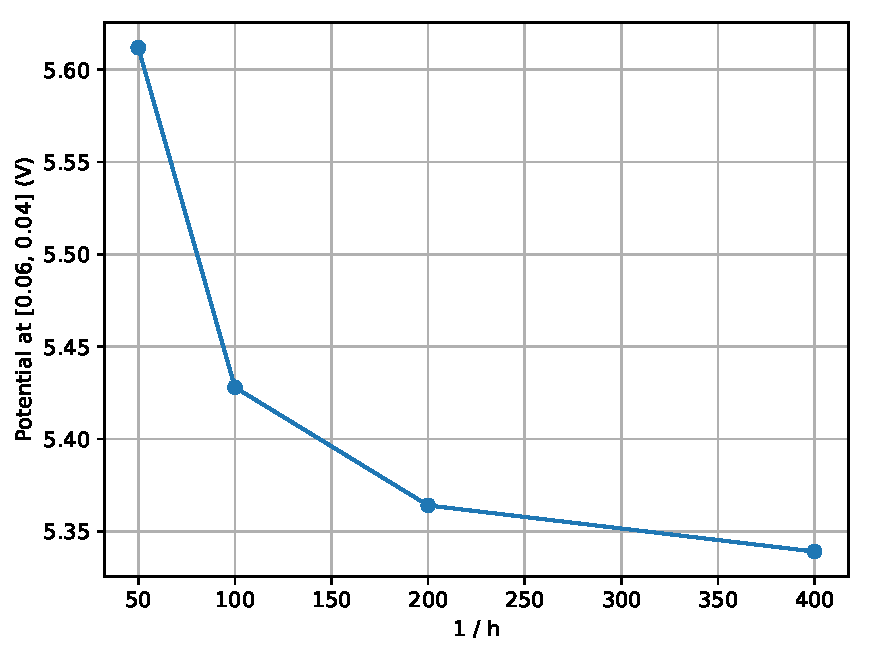
\includegraphics[width=\columnwidth]{plots/q3c_potential.pdf}
		\caption
		{Potential at (0.06, 0.04) found by SOR versus $1/h$. Note that $\omega=1.3$.}
		\label{fig:q3c_potential}
	\end{figure}
	
	\subsection{Jacobi Method}
	% Use the Jacobi method to solve this problem for the same values of h used in part (c). Tabulate and plot the values of the potential at (x, y) = (0.06, 0.04) versus 1/h and the number of iterations versus 1/h. Comment on the properties of both plots and compare to those of SOR.
	
	The number of iterations of the Jacobi method versus $1/h$ is tabulated in \autoref{table:q3d_iterations} and plotted in \autoref{fig:q3d_iterations}. Similarly to SOR, the smaller the node spacing is, the more iterations the program will take to run. We can see however that the Jacobi method takes a much larger number of iterations to converge. Theoretically, the Jacobi method should have a time complexity of $O(N^4)$. However, the experimental data shows a complexity closer to $O(1/h^3) = O(N^3)$. The discrepancy can perhaps be because of the relatively small amount of data points.
	
	\begin{table}[!htb]
		\centering
		\caption{Number of iterations versus $\omega$ when using the Jacobi method.}
		\csvautobooktabular{csv/q3d_iterations.csv}
		\label{table:q3d_iterations}
	\end{table}

	\begin{figure}[!htb]
		\centering
		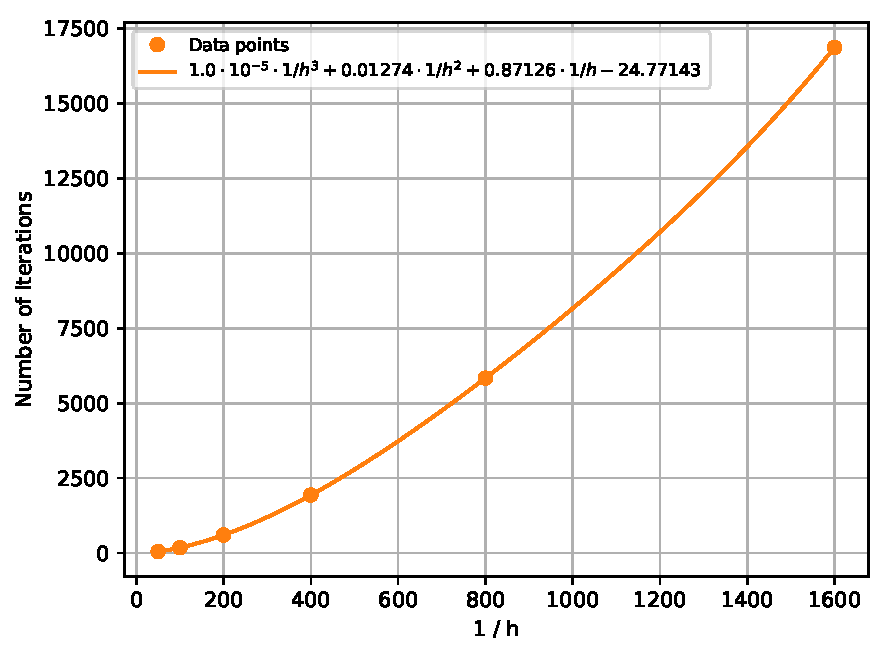
\includegraphics[width=\columnwidth]{plots/q3d_iterations.pdf}
		\caption
		{Number of iterations of the Jacobi method versus $1/h$.}
		\label{fig:q3d_iterations}
	\end{figure}

	The potential values found at (0.06, 0.04) versus $1/h$ with the Jacobi method are tabulated in \autoref{table:q3d_potential} and plotted in \autoref{fig:q3d_potential}. These potential values are almost identical to the SOR ones. Similarly to SOR, the smaller the node spacing is, the more accurate the calculated potential is.

	\begin{table}[!htb]
		\centering
		\caption{Potential at (0.06, 0.04) versus $1/h$ when using the Jacobi method.}
		\csvautobooktabular{csv/q3d_potential.csv}
		\label{table:q3d_potential}
	\end{table}

	\begin{figure}[!htb]
		\centering
		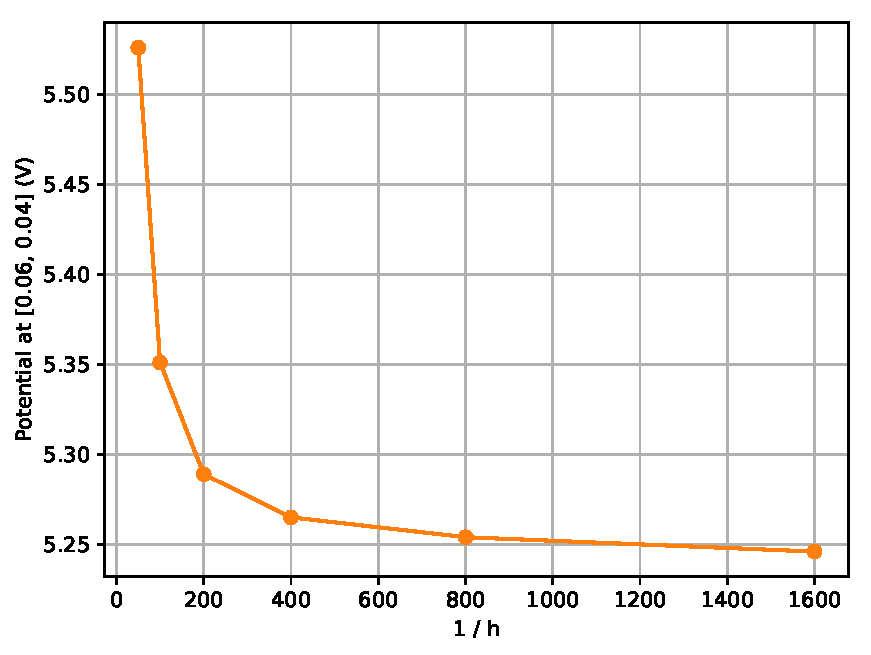
\includegraphics[width=\columnwidth]{plots/q3d_potential.pdf}
		\caption
		{Potential at (0.06, 0.04) versus $1/h$ when using the Jacobi method.}
		\label{fig:q3d_potential}
	\end{figure}

	The number of iterations of both SOR and the Jacobi method can be seen in \autoref{fig:q3d_iterations_comparison}, which shows the clear benefits of SOR.

	\begin{figure}[!htb]
		\centering
		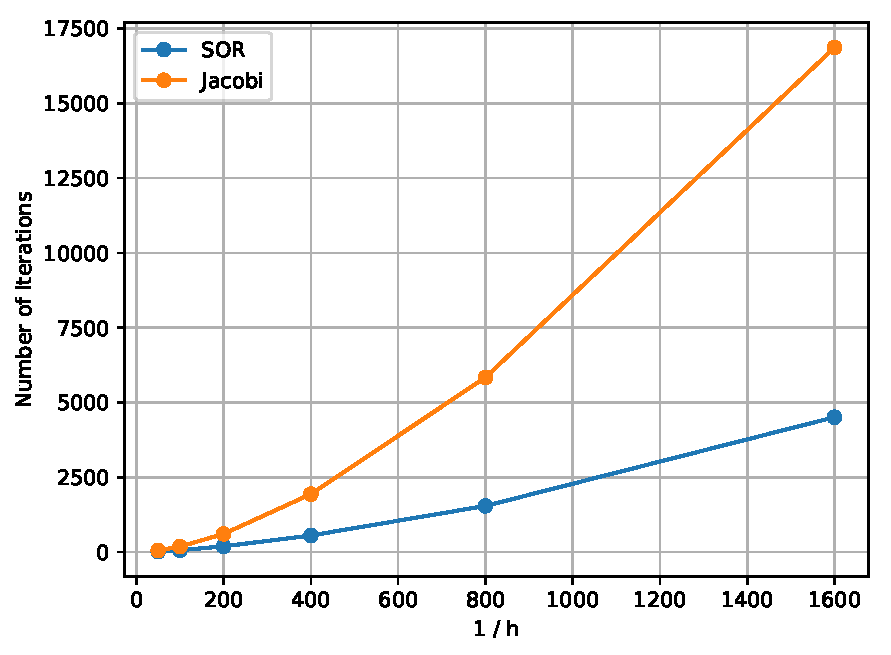
\includegraphics[width=\columnwidth]{plots/q3d_iterations_comparison.pdf}
		\caption
		{Comparison of number of iterations when using SOR and Jacobi methods versus $1/h$. Note that $\omega=1.3$ for the SOR program.}
		\label{fig:q3d_iterations_comparison}
	\end{figure}
	
	\subsection{Non-uniform Node Spacing}
	% Modify the program you wrote in part (a) to use the five-point difference formula derived in	class for non-uniform node spacing. An alternative to using equal node spacing, h, is to use	smaller node spacing in more “difficult” parts of the problem domain. Experiment with a	scheme of this kind and see how accurately you can compute the value of the potential at (x, y)	= (0.06, 0.04) using only as many nodes as for the uniform case h = 0.01 in part (c).
	
	First, we adjust the equation derived in class to set $a_1 = \Delta_x\alpha_1$, $a_2 = \Delta_x\alpha_2$, $b_1 = \Delta_y\beta_1$ and $b_2 = \Delta_y\beta_2$. These values correspond to the distances between adjacent nodes \footnote{Note that, in the program, index $i$ is associated to position $x$ and index $j$ is associated to position $y$. This is purely for easier handling of the matrices.}, and can be easily calculated by the program. Then, the five-point difference formula for non-uniform spacing can be seen in \autoref{eq:non_uniform}.
	
	\begin{align} \label{eq:non_uniform}
		\begin{split}
			\phi^{k + 1}_{i,j} = 
			&\frac{1}{a_1 + a_2}\left(\frac{\phi^k_{i - 1,j}}{a_1} + \frac{\phi^k_{i + 1,j}}{a_2}\right) + \\
			&\frac{1}{b_1 + b_2}\left(\frac{\phi^k_{i, j - 1}}{b_1} + \frac{\phi^k_{i, j + 1}}{b_2}\right)
		\end{split}
	\end{align}
	
	This was implemented in the finite difference program, as seen in \mintinline{python}{NonUniformRelaxer} class in the \mintinline{python}{finite_diff.py} file shown in \autoref{lst:finite_diff}. As can be seen in this code, many different mesh arrangements were tested. The arrangement that was chosen can be seen in \autoref{fig:q3e}. This arrangement was chosen because the ``difficult'' regions are close to the inner conductor, where there is a higher concentration of nodes. The potential at (0.06, 0.04) obtained from this arrangement is \SI{5.243}{\volt}, which seems like an accurate potential value. Indeed, as can be seen in \Cref{fig:q3c_potential,fig:q3d_potential}, the potential value for small node spacings tends towards \SI{5.24}{\volt} for both the Jacobi and SOR methods.
	
	\begin{figure}[!htb]
		\centering
		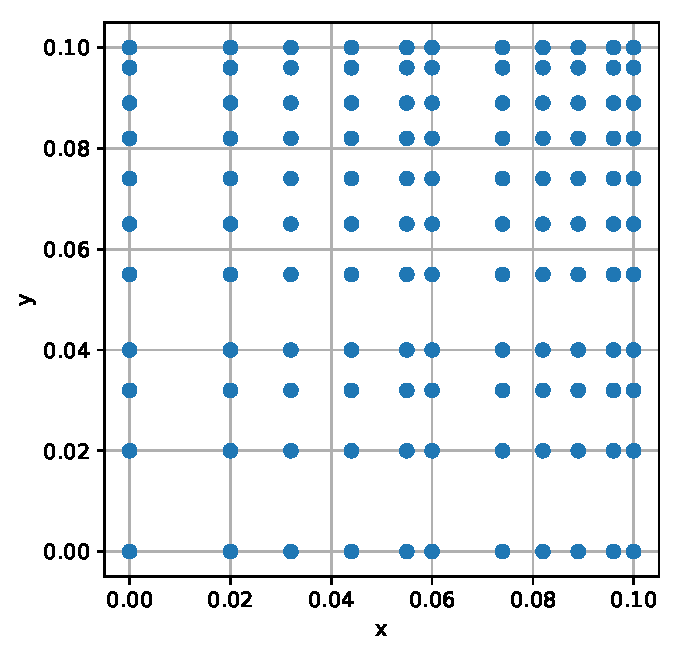
\includegraphics[width=\columnwidth]{plots/q3e.pdf}
		\caption
		{Final mesh arrangement used for non-uniform node spacing. Each point corresponds to a mesh point. Points are positioned closer to the inner conductor, since this is a more difficult area.}
		\label{fig:q3e}
	\end{figure}

	\section*{Conclusion}
	
	A Choleski matrix solver, finite difference mesh generator, and finite difference potential solver were created with positive results. The trade-offs between the various implementations of the algorithms associated with these programs were explored and analyzed.
	
	\onecolumn
	
%	\appendix
	
	\begin{appendices}
		
		\section{Code Listings} \label{appendix:code}
		
		\setminted{linenos,breaklines,fontsize=\footnotesize}
		
		\begin{center}
			\captionof{listing}{Custom matrix package (\texttt{matrices.py}).}
			\inputminted{python}{../matrices.py}
			\label{lst:matrices}
		\end{center}
		
		\begin{center}
			\captionof{listing}{CSV manipulation utilities (\texttt{csv\_saver.py}).}
			\inputminted{python}{../csv_saver.py}
			\label{lst:csv_saver}
		\end{center}
		
		\begin{center}
			\captionof{listing}{Choleski decomposition (\texttt{choleski.py}).}
			\inputminted{python}{../choleski.py}
			\label{lst:choleski}
		\end{center}
		
		\begin{center}
			\captionof{listing}{Linear resistive networks (\texttt{linear\_networks.py}).}
			\inputminted{python}{../linear_networks.py}
			\label{lst:linear_networks}
		\end{center}
		
		\begin{center}
			\captionof{listing}{Question 1 (\texttt{q1.py}).}
			\inputminted{python}{../q1.py}
			\label{lst:q1}
		\end{center}
		
		\begin{center}
			\captionof{listing}{Question 2 (\texttt{q2.py}).}
			\inputminted{python}{../q2.py}
			\label{lst:q2}
		\end{center}
		
		\begin{center}
			\captionof{listing}{Finite difference method (\texttt{finite\_diff.py}).}
			\inputminted{python}{../finite_diff.py}
			\label{lst:finite_diff}
		\end{center}
		
		\begin{center}
			\captionof{listing}{Question 3 (\texttt{q3.py}).}
			\inputminted{python}{../q3.py}
			\label{lst:q3}
		\end{center}
		
		\section{Output Logs} \label{appendix:logs}
		
		\begin{center}
			\captionof{listing}{Output of Question 1 program (\texttt{q1.txt}).}
			\inputminted{pycon}{logs/q1.txt}
			\label{lst:q1_log}
		\end{center}
		
		\begin{center}
			\captionof{listing}{Output of Question 2 program (\texttt{q2.txt}).}
			\inputminted{pycon}{logs/q2.txt}
			\label{lst:q2_log}
		\end{center}
		
		\begin{center}
			\captionof{listing}{Output of Question 3 program (\texttt{q3.txt}).}
			\inputminted{pycon}{logs/q3.txt}
			\label{lst:q3_log}
		\end{center}
	\end{appendices}

\end{document}
